%\nonstopmode
\documentclass[aspectratio=169]{beamer}
\usepackage[utf8]{inputenc}
% \usepackage[frenchb]{babel}
\usepackage{amsmath}
\usepackage{mathtools}
\usepackage{breqn}
\usepackage{multirow}
\usetheme{boxes}
\usepackage{graphicx}
%\useoutertheme[footline=authortitle,subsection=false]{miniframes}

\beamertemplatenavigationsymbolsempty

\definecolor{TitleOrange}{RGB}{255,137,0}
\setbeamercolor{title}{fg=TitleOrange}
\setbeamercolor{frametitle}{fg=TitleOrange}

\definecolor{ListOrange}{RGB}{255,145,5}
\setbeamertemplate{itemize item}{\color{ListOrange}$\blacktriangleright$}

\definecolor{verygrey}{RGB}{70,70,70}
\setbeamercolor{normal text}{fg=verygrey}


\usepackage{tabu}
\usepackage{multicol}
\usepackage{vwcol}
\usepackage{stmaryrd}
\usepackage{graphicx}

\usepackage[normalem]{ulem}

\title{Introducing Garage}
\subtitle{a new storage platform for self-hosted geo-distributed clusters}
\author{Deuxfleurs Association}
\date{FOSDEM '22}

\begin{document}

\begin{frame}
	\centering
	
\includegraphics[width=.3\linewidth]{../../sticker/Garage.pdf}
	\vspace{1em}

	{\large\bf Deuxfleurs Association}
	\vspace{1em}

	\url{https://garagehq.deuxfleurs.fr/}

	Matrix channel: \texttt{\#garage:deuxfleurs.fr}
\end{frame}

\begin{frame}
	\frametitle{Our objective at Deuxfleurs}
	
	\begin{center}
		\textbf{Promote self-hosting and small-scale hosting\\
			as an alternative to large cloud providers}
	\end{center}
	\vspace{2em}
	\visible<2->{
		Why is it hard?
	}
	\visible<3->{
		\vspace{2em}
		\begin{center}
			\textbf{\underline{Resilience}}\\
			{\footnotesize (we want good uptime/availability with low supervision)}
		\end{center}
	}
\end{frame}

\begin{frame}
	\frametitle{How to be resilient (the hard way)}

	Entreprise-grade systems typically employ:
	\vspace{1em}
	\begin{itemize}
		\item RAID
		\item Redundant power grid + UPS
		\item Redundant Internet connections
		\item Low-latency links
		\item ... 
	\end{itemize}
	\vspace{1em}
	$\to$ it's costly and only worth it at DC scale
\end{frame}

\begin{frame}
	\frametitle{How to be resilient (the \underline{\textbf{cheap}} way)}

	\only<1,4-5>{
		Instead, we use:
		\vspace{1em}
		\begin{itemize}
			\item \textcolor<2->{gray}{Commodity hardware (e.g. old desktop PCs)}
				\vspace{.5em}
			\item<4-> \textcolor<5->{gray}{Commodity Internet (e.g. FTTB, FTTH) and power grid}
				\vspace{.5em}
			\item<5-> \textcolor<6->{gray}{\textbf{Geographical redundancy} (multi-site replication)}
		\end{itemize}
	}
	\only<2>{
		\begin{center}
			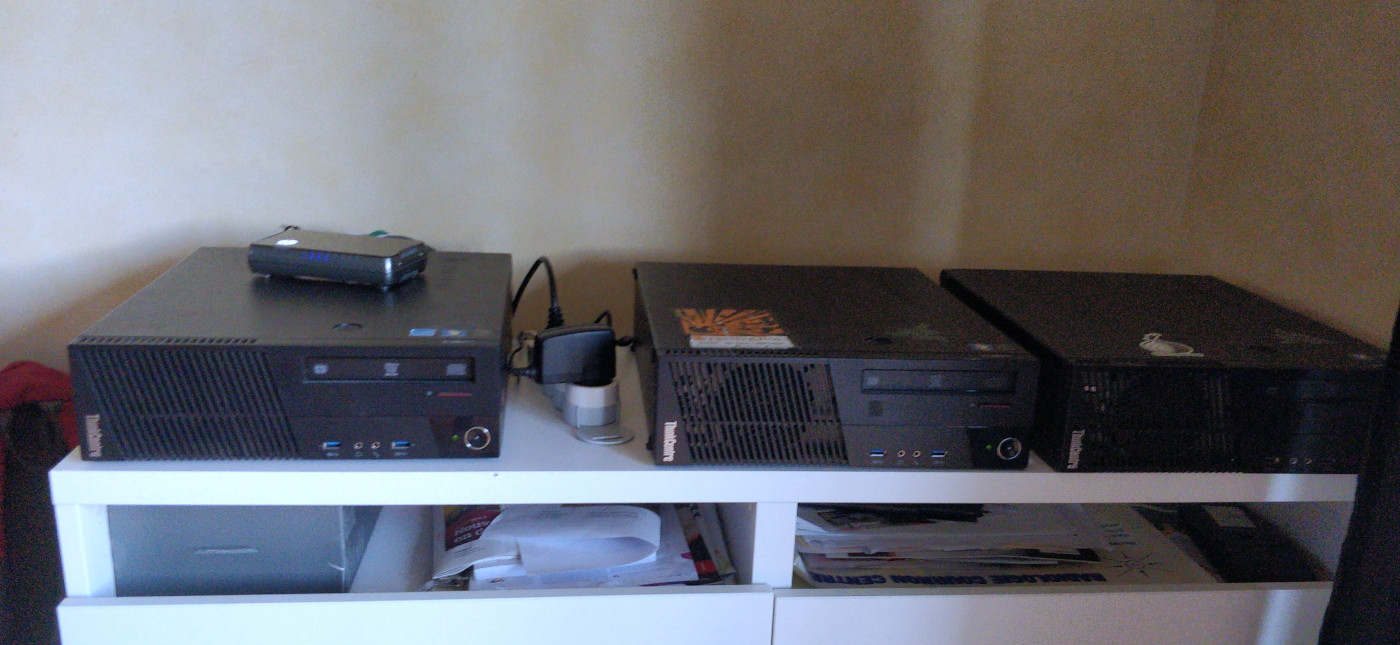
\includegraphics[width=.8\linewidth]{assets/atuin.jpg}
		\end{center}
	}
	\only<3>{
		\begin{center}
			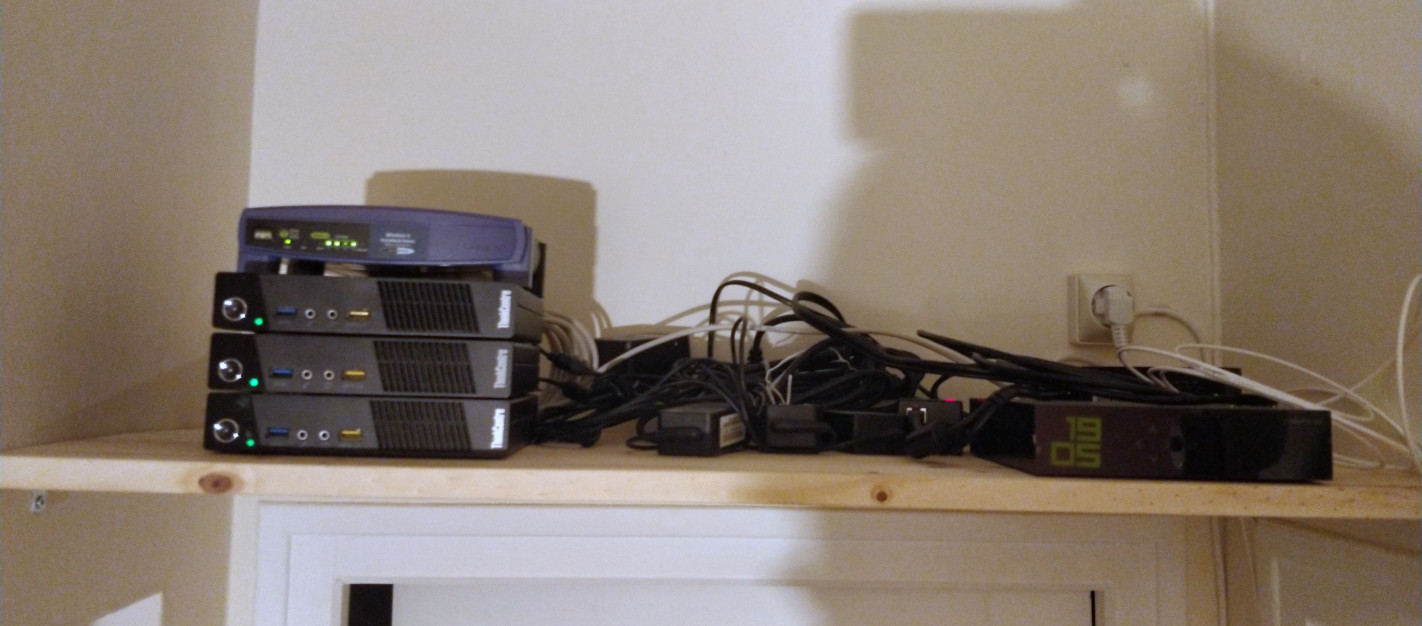
\includegraphics[width=.8\linewidth]{assets/neptune.jpg}
		\end{center}
	}
	\only<6>{
		\begin{center}
			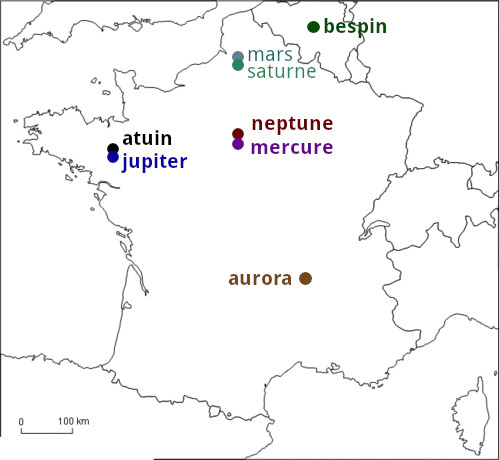
\includegraphics[width=.5\linewidth]{assets/inframap.jpg}
		\end{center}
	}
\end{frame}

\begin{frame}
	\frametitle{How to make this happen}
	\begin{center}
		\only<1>{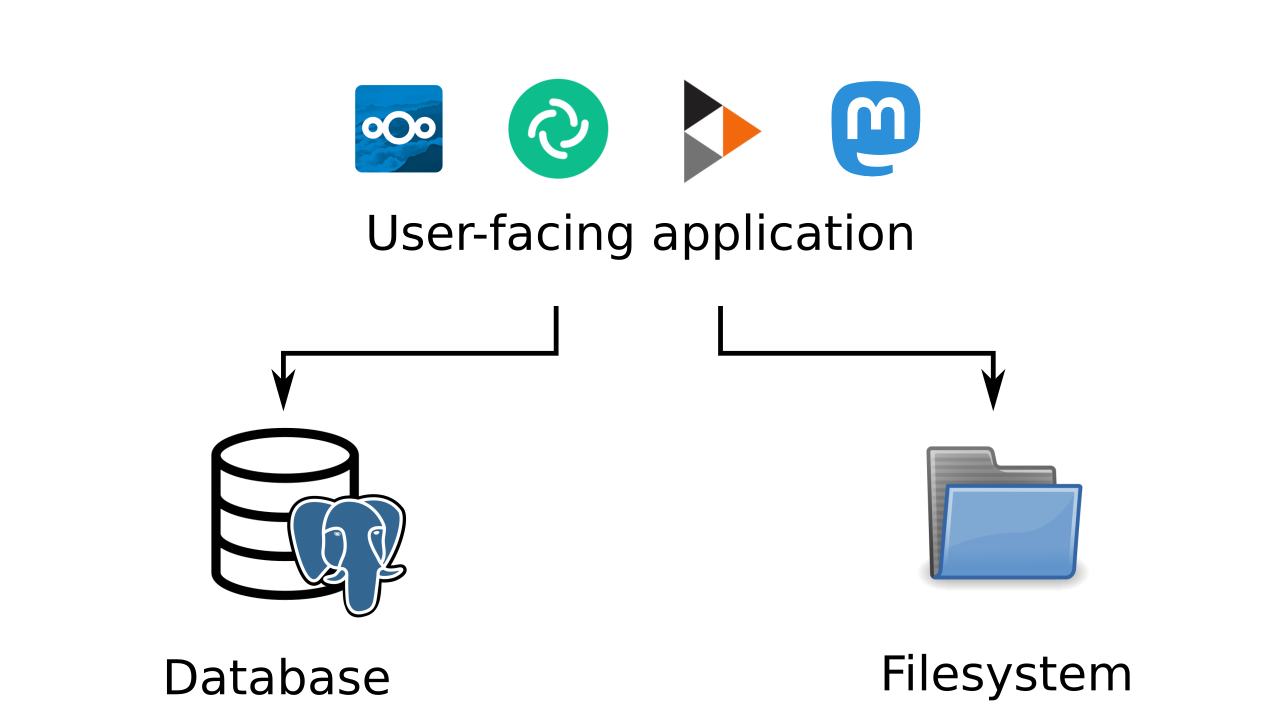
\includegraphics[width=.8\linewidth]{assets/slide1.png}}%
		\only<2>{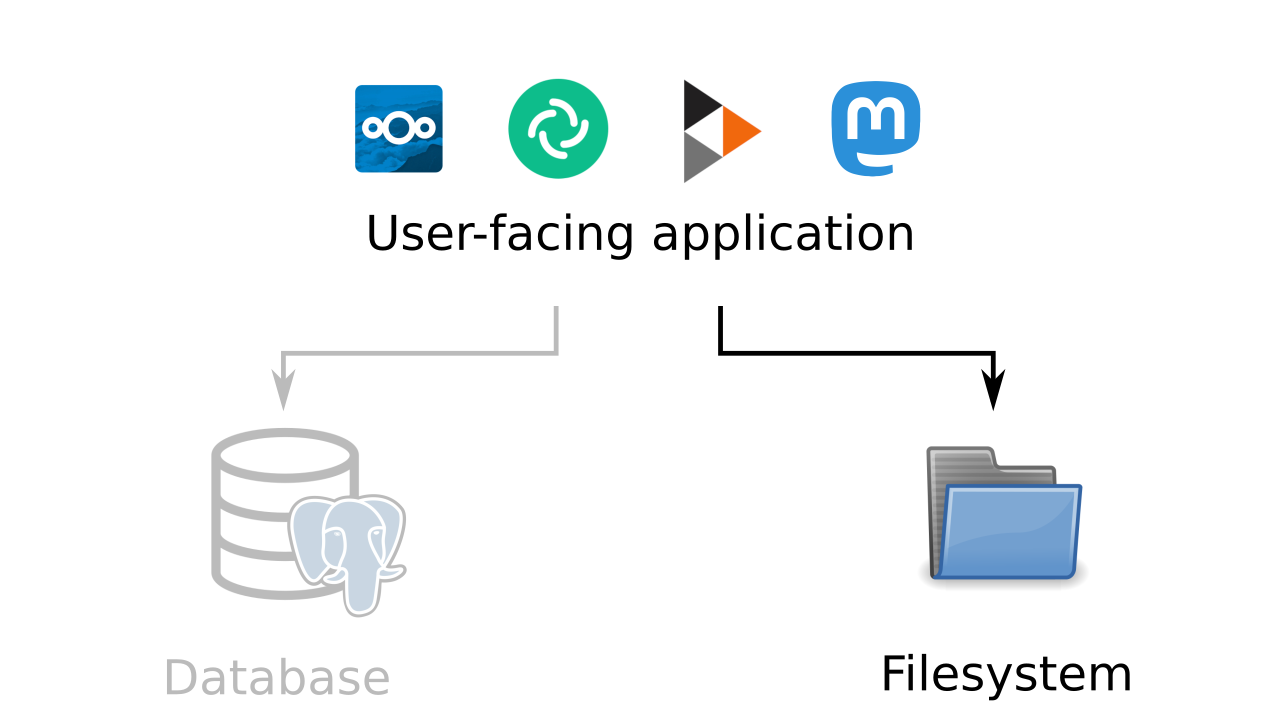
\includegraphics[width=.8\linewidth]{assets/slide2.png}}%
		\only<3>{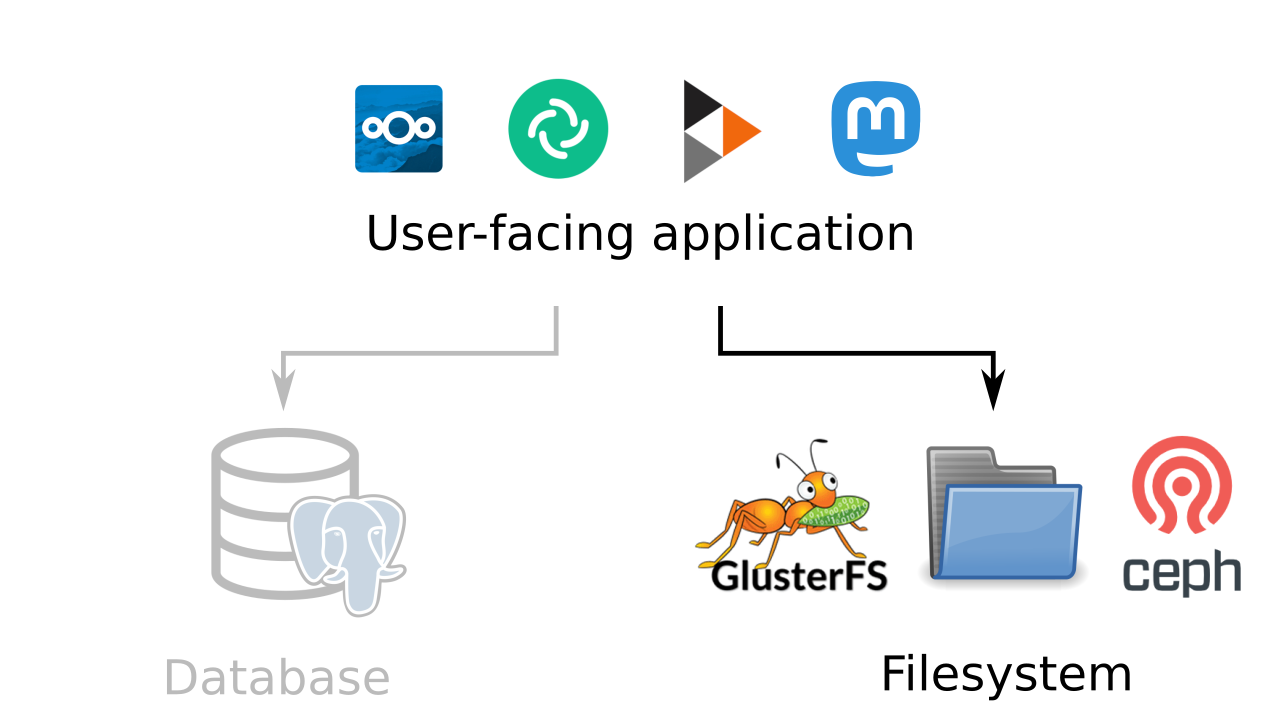
\includegraphics[width=.8\linewidth]{assets/slide3.png}}%
	\end{center}
\end{frame}

\begin{frame}
	\frametitle{Distributed file systems are slow}
	File systems are complex, for example:
	\vspace{1em}
	\begin{itemize}
		\item Concurrent modification by several processes
			\vspace{1em}
		\item Folder hierarchies
			\vspace{1em}
		\item Other requirements of the POSIX spec
	\end{itemize}
	\vspace{1em}
	Coordination in a distributed system is costly

	\vspace{1em}
	Costs explode with commodity hardware / Internet connections\\
	{\small (we experienced this!)}
\end{frame}

\begin{frame}
	\frametitle{A simpler solution: object storage}
	Only two operations:
	\vspace{1em}
	\begin{itemize}
		\item Put an object at a key
			\vspace{1em}
		\item Retrieve an object from its key
	\end{itemize}
	\vspace{1em}
	{\footnotesize (and a few others)}

	\vspace{1em}
	Sufficient for many applications!
\end{frame}

\begin{frame}
	\frametitle{A simpler solution: object storage}
		\begin{center}
			
\includegraphics[width=.2\linewidth]{../2020-12-02_wide-team/img/Amazon-S3.jpg}
			\hspace{5em}
			
\includegraphics[width=.2\linewidth]{assets/minio.png}
		\end{center}
		\vspace{1em}
	S3: a de-facto standard, many compatible applications

	\vspace{1em}

	MinIO is self-hostable but not suited for geo-distributed deployments
\end{frame}


\begin{frame}
	\frametitle{But what is Garage, exactly?}
	\textbf{Garage is a self-hosted drop-in replacement for the Amazon S3 object store}\\
	\vspace{.5em}
	that implements resilience through geographical redundancy on commodity hardware
		\begin{center}
			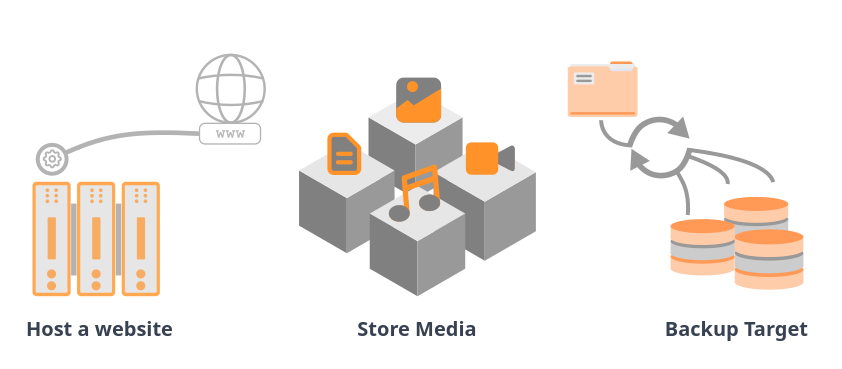
\includegraphics[width=.8\linewidth]{assets/garageuses.png}
		\end{center}
\end{frame}

\begin{frame}
	\frametitle{What makes Garage different?}
	\textbf{Coordination-free:}
			\vspace{2em}
	\begin{itemize}
		\item No Raft or Paxos
			\vspace{1em}
		\item Internal data types are CRDTs
			\vspace{1em}
		\item All nodes are equivalent (no master/leader/index node)
	\end{itemize}
			\vspace{2em}
	$\to$ less sensitive to higher latencies between nodes
\end{frame}

\begin{frame}
	\frametitle{What makes Garage different?}
		\begin{center}
			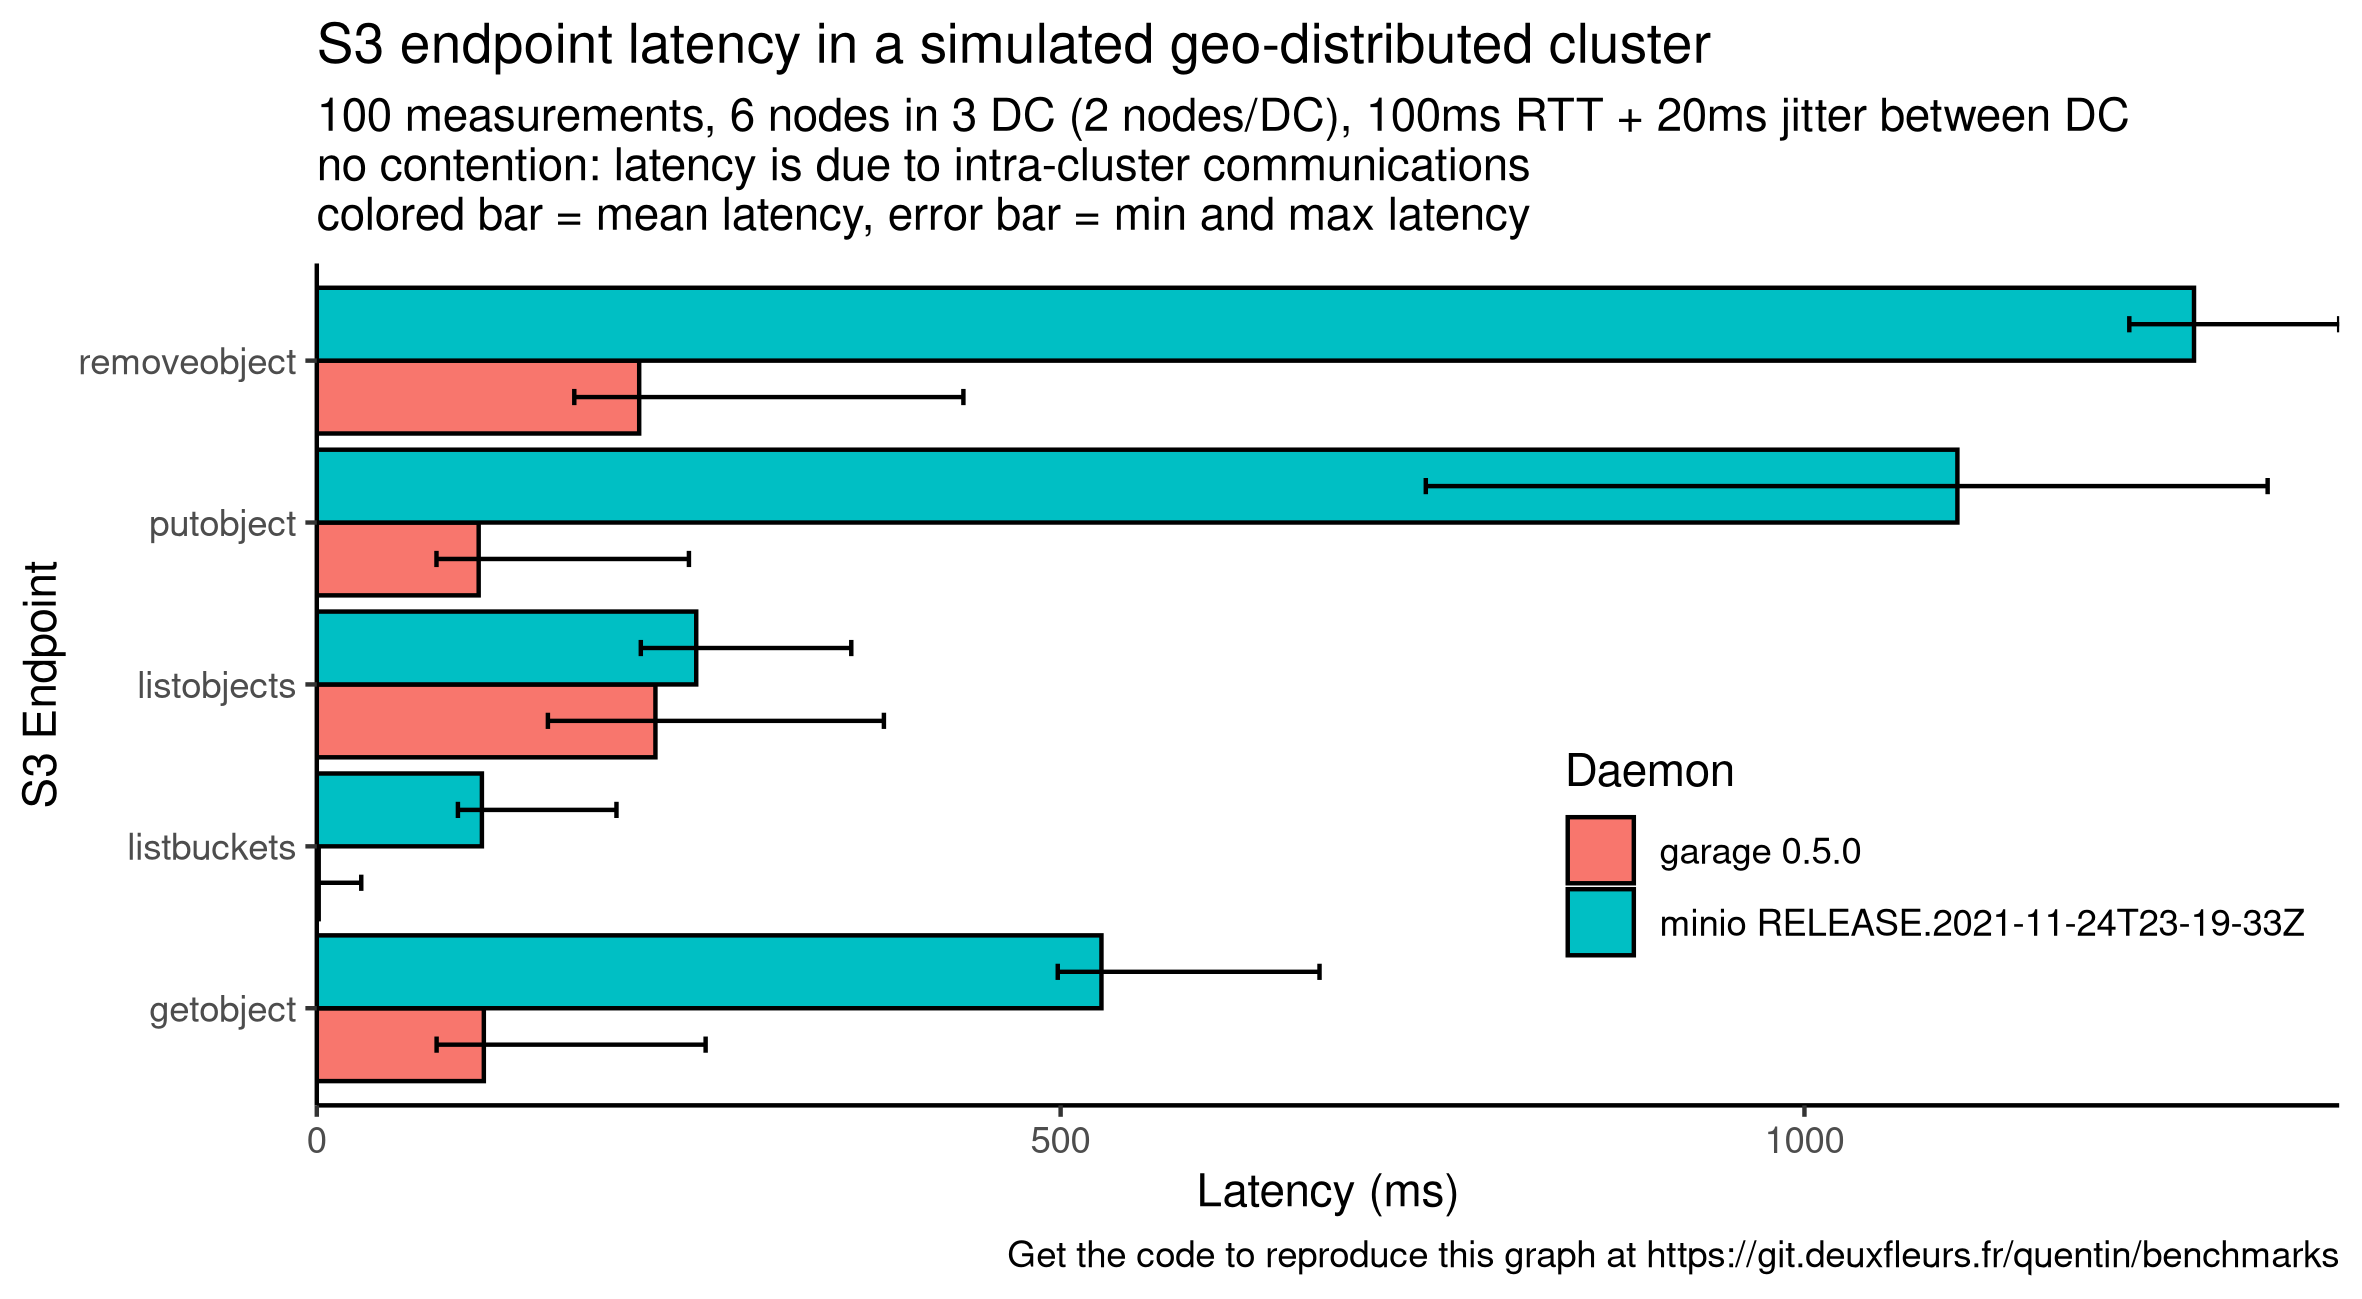
\includegraphics[width=.9\linewidth]{assets/endpoint-latency-dc.png}
		\end{center}
\end{frame}

\begin{frame}
	\frametitle{What makes Garage different?}
	\textbf{Consistency model:}
			\vspace{2em}
	\begin{itemize}
		\item Not ACID (not required by S3 spec) / not linearizable
			\vspace{1em}
		\item \textbf{Read-after-write consistency}\\
			{\footnotesize (stronger than eventual consistency)}
	\end{itemize}
\end{frame}

\begin{frame}
	\frametitle{What makes Garage different?}
	\textbf{Location-aware:}
	\vspace{2em}
		\begin{center}
			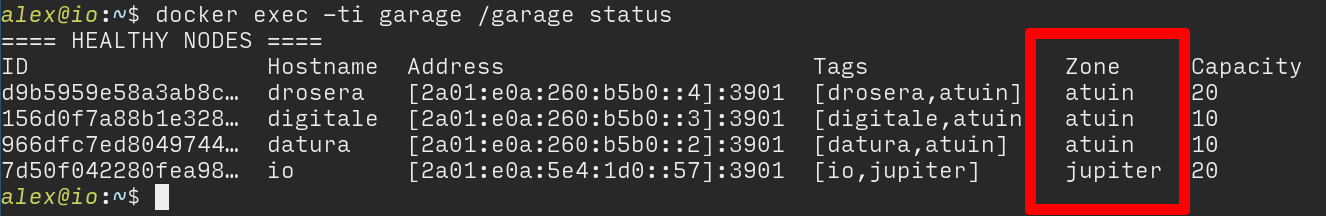
\includegraphics[width=\linewidth]{assets/location-aware.png}
		\end{center}
	\vspace{2em}
	Garage replicates data on different zones when possible
\end{frame}

\begin{frame}
	\frametitle{What makes Garage different?}
		\begin{center}
			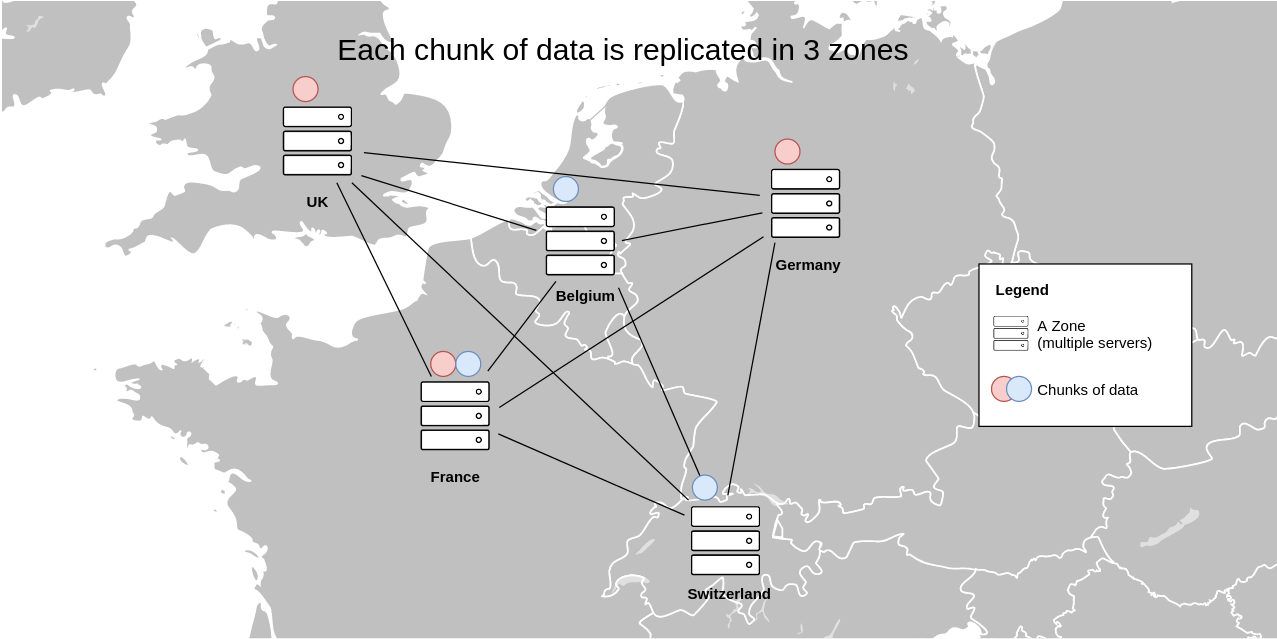
\includegraphics[width=.8\linewidth]{assets/map.png}
		\end{center}
\end{frame}

\begin{frame}
	\frametitle{An ever-increasing compatibility list}
		\begin{center}
			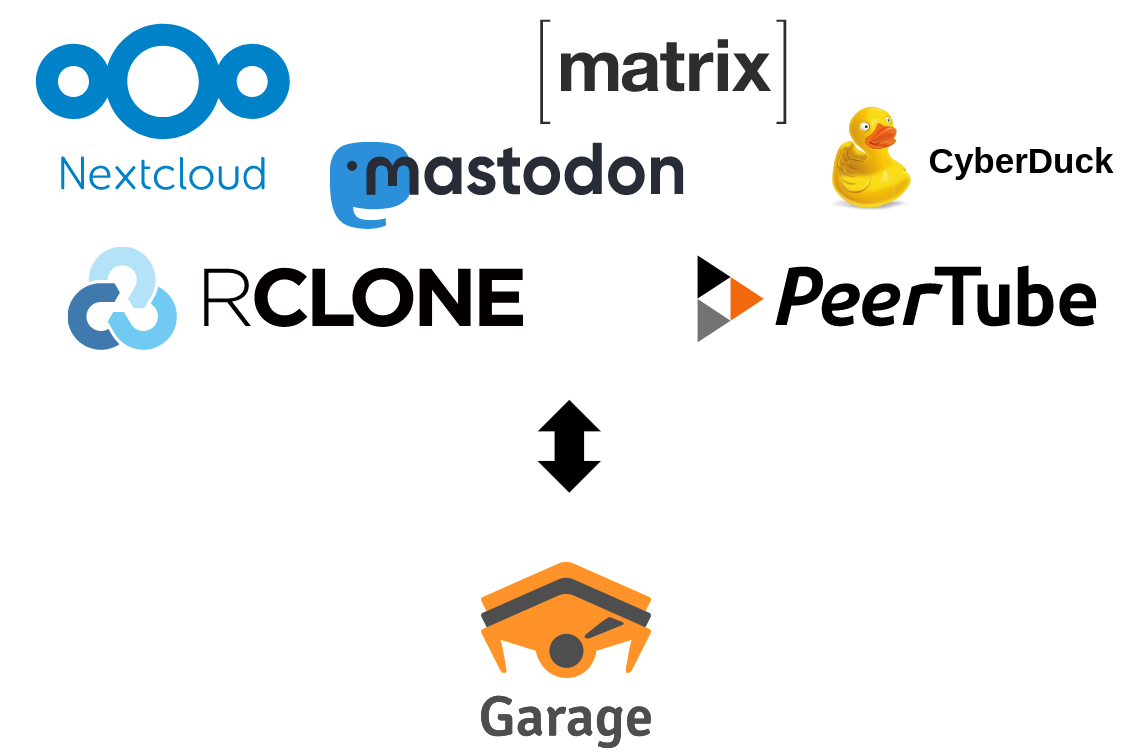
\includegraphics[width=.7\linewidth]{assets/compatibility.png}
		\end{center}
\end{frame}

\begin{frame}
	\frametitle{Get Garage now!}
	\begin{center}
			
\includegraphics[width=.3\linewidth]{../../logo/garage_hires.png}\\
			\vspace{-1em}
		\url{https://garagehq.deuxfleurs.fr/}\\
		Matrix channel: \texttt{\#garage:deuxfleurs.fr}

		\vspace{2em}
			
\includegraphics[width=.09\linewidth]{assets/rust_logo.png}
			
\includegraphics[width=.2\linewidth]{assets/AGPLv3_Logo.png}
	\end{center}
\end{frame}

\begin{frame}
	\frametitle{Demo time!}
\end{frame}

\end{document}

%% vim: set ts=4 sw=4 tw=0 noet spelllang=fr :
